\chapter{Chronos hardware}

\section{Contents of the chapter}

In this chapter we'll describe the hardware features witch are
available in the chronos watch. We assume that the reader is
interested in the applications watch can be put to, but these are
limited by the hardware capabilities. Thus understanding what the
hardware can do (and what it can't do) for us is the first step to
understanding what applications are possible and may be supported by
the platform.

The descriptions will be short and high level, aiming rather to
introduce the functionality and possibilities than boring into specific
details.

\section{eZ430-Chronos package from Texas Instruments}

The eZ430 Chronos is a reference platform for wireless mobile systems.
It is a versatile, highly integrated smart watch.  According to
manufacturer, Texas Instrument, this product was designed for
developers as an evaluation platform.  Although, it is not intended
for consumer market, it is widely available and popular among
technology hobbyists.

It is sold in a box that contains the watch, USB programing dongle and
USB radio dongle along with software disc and a screw driver. These
are shown on figures \ref{fig:chronos_kit} and \ref{fig:chronos_watch}.
The programming dongle is the upper right and radio dongle in
lower right part of figure \ref{fig:chronos_watch}.

\begin{figure}[h]
  \centering
  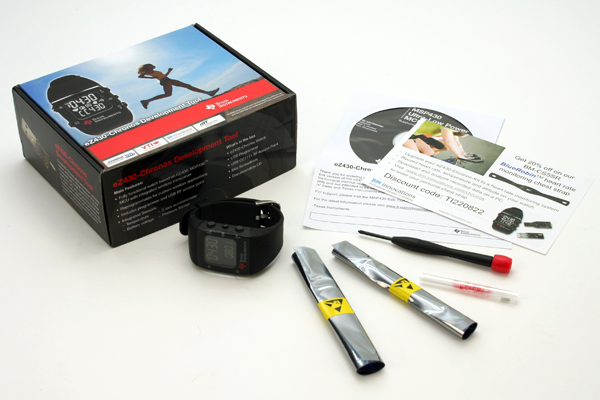
\includegraphics[width=0.7\textwidth]{img/chronos_kit.jpg}
  \caption{Contents of the chronos kit. (Courtesy Texas Instruments)}
  \label{fig:chronos_kit}
\end{figure}

\begin{figure}[h]
  \centering
  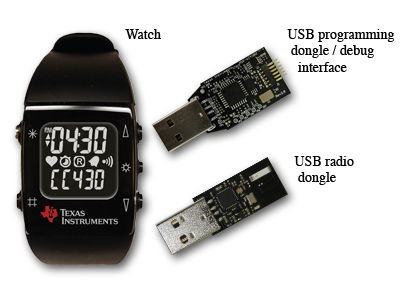
\includegraphics[width=0.6\textwidth]{img/chronos_watch.png}
  \caption{Main elements of the chronos kit. (Courtesy Texas
  Instruments)}
  \label{fig:chronos_watch}
\end{figure}

\section{Elements of the watch}
Chronos watch is battery powered and has a typical wrist strap that
allows to wear it like any other watch. It's uniqueness however comes
from what lies within the waterproof housing. Of the more common
elements it has a {\bf 96 segment LCD display}, which includes two
rows of digits, respectively 4 and 5 digits long, and many other
symbols. All segments can be lit (and even blinked) independently.
This allows to display crude letters along with numbers. Available
segments are shown in figure \ref{fig:chronos_segs}.  Watch also has 5
programmable buttons, one of which controls the screen back-light.

\begin{figure}[h]
  \centering
  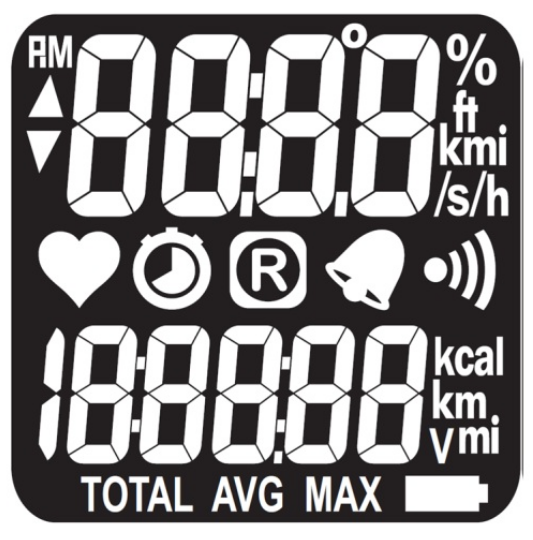
\includegraphics[width=0.4\textwidth]{img/chronos_segs.png}
  \caption{All segments of the LCD display. (Courtesy Texas
  Instruments)}
  \label{fig:chronos_segs}
\end{figure}

What's less common is it's MCU ({\bf Mobile Compute Unit}) labeled
CC430F6137 that can be fully programmed by the user. This MCU is a, so
called, system-on-chip (or SoC), because it contains a built in {\bf
radio transceiver}. Conveniently it uses 868 MHz radio waves, a band
for which license is not required (2.4 GHz, that WiFi for instance
uses, is another exception). The MCU will be further explored below.
Watch also has some on-board sensors.  One is an {\bf accelerometer}
and other a {\bf temperature and pressure sensor}. The accelerometer
can detect watch position relative to the earth's gravity, notice
sudden motion and also detect if watch is in free fall. The
thermometer is quite typical, being able to measure current air
temperature. Pressure sensor however is precise enough to measure even
a 0.3 meter change in altitude. That's enough to detect on which floor
of a building you are. Thus it's often called an {\bf altimeter}.

Finally, the watch casing is water resistant up to 30 meters and typical
CR2032 batteries, used in chronos, have capacity of 225 mAh and
provide nominal voltage of 3.0 V.

\section{Mobile Compute Unit}

MCU is a Compute Programmable Unit (CPU) designed for extremely
low-power usage. The one used in chronos has the MSP430 (Mixed Signal
microProcessor) architecture particularly suited for such
applications. It belongs to the TI family of products code named CC430
which features 16-bit, RISC based (Reduced Instruction Set Computing)
CPUs and is described in datasheet \cite{CC430ds}. The exact chip
soldered in the watch is CC430F6137 and it's datasheet
\cite{CC430F6137ds} only describes details specific to this particular
chip.

Applications that may be ran on the watch are limited by MCU's
resources. Most limiting one is the memory. There are two types
available:
\begin{itemize}
  \item {\bf 32KB of flash memory}. This is a non-volatile fast-read
    slow-write on-chip memory. It stores code and data. After reset
    MCU jumps to a location (address 0x8000) in this memory and starts
    executing instructions recorded there. It's amount may seem little
    but with
    modern code-size optimizing compilers quite complex applications
    are possible. For example this is just enough memory to fit a
    temperature monitoring application in which each node sends out
    it's readings and forwards ridings of other nodes in a way that
    enables results to reach a single sink node.
  \item {\bf 4KB of RAM} It is very similar to PC RAM and it's
    operation consumes a lot of energy. That's why it's amount is so
    small. 4KB is however just enough to fit the temperature monitoring
    application mentioned above.
\end{itemize}

The MCU clock is scalable and can run at {\bf maximum frequency of 20 MHz}.
MSP430 RISC instructions are however much simpler than, for example
x86 ones. To give a feel for this difference, 16 MHz (default in
chronos) was compared to an Intel Core 2 x86 processor. ..
<Floyd-Warshal comparison> % TODO(horban): Dorobic test szybkosci

\section{Additional hardware functions}

There are certain functions that, though possible to implement in
software are also easily implemented in hardware. Choosing the second
approach saves both execution time and energy.  Also some features can
only be implemented with hardware support.  Here we'll walk through
most important ones available in the CC430f6137 MCU (and many other
members of the CC430 family for that matter).

{\bf LPM (Low Power Mode) support} allows MCU to dynamically switch to
one of several power states.  They are called Active, LPM0, LPM1, etc.
Each successive one consumes less energy, by disabling more hardware
functions and peripherals. This mechanism is crucial for lengthening
the battery life. To give the reader a better feel of how important
that is, we list some crude battery life estimates:

\begin{itemize}
    \item In Active mode (executing instructions) watch battery would
    last for a week (6.8 days).
    \item In LPM0 or LPM1 this would grow to roughly 280 days.
    \item In LPM2 battery would last around 9 years.
    \item And finally in LPM3 or LPM4 if would last half a decade (52
    years) which is more than battery shelf-life.
\end{itemize}
From this, it's plain that if the battery is to last years, MCU must
spend most of the time in lowest power modes.

For this reason, another vital subsystem is the {\bf Timer\_A} which
allows to sets an alarm that will fire (interrupt) after specific
period of time (on the order of milliseconds) and execute certain
piece of code (interrupt handler). It would be impossible to use low
power modes without such functionality.

We should not forget that primarily our device is a watch. Thus a {\bf
RTC\_A (Real Time Clock)} is provided. This module provides a
wall-like clock and calendar functions. It is the best way to access
seconds, minutes, hours, day of week, day of month, month, and year.
Moreover it can also be configured as a general-purpose counter -
something similar to Timer\_A.

The MCU has pins coming out of it's chip. Most of them are called {\bf
IO pins}. They can be configured to act as an input, output or special
function.  In input mode they inform of the signal that's connected to
them (high or low). Similarly in output mode they can generate high or
low signal \footnote{You may be tempted to connect such input and
output pins to experiment with signal passing. Doing so is dangerous!
Output pin will produce maximum of several mA of current. Input pin
will try to accept all this current. Thus such a connection without a
resistor results in a short circuit {\bf through the chip}. Use 2k
$\Omega$ resistor to be safe.}. Special function mode connects the pin
to an internal hardware component i.e.  the LCD driver.  Also it is
possible to be notified (interrupt) if state of an input pin changes.
This gives a good way to implement buttons.

Now you may have noticed that there are many more LCD segments on the
display than there are pins on the chip. Even if there were enough,
using so many pins for the LCD would be wasteful. It's better to
spread the data over time. In a technique called multiplexing, the
chip selects a group of segments powering a control pin and lits ones
within this group. 8 group pins and 8 element pins are enough to drive
64 segments in this fashion. Groups are changed quickly enough that human
won't notice the blinking which makes it a very practical solution.
However doing this in software would be very wasteful so the {\bf
LCD\_B} hardware driver does all this for us instead.

Another vital hardware driver is called {\bf USCI (Universal Serial
Communication Interface)}. It can be configured to pose as one of
standardised communication interfaces. Most notably these are SPI
(Serial Peripheral Interface), I$^2$C (Inter-Integrated Circuit) and
UART (Universal Asynchronous Receiver/Transmitter). Though cumbersome,
each one can be implemented in software, however hardware support
increases performance by an order of magnitude. Mentioned UART is
particularly important during development, because it allows sending
text from watch MCU to a PC.

An interesting and very practical feature of the CC430 family is
their ability to do {\bf port remapping} in runtime. Typically special
functions are hard-connected to certain chip pins. I.e. UART's Tx and
Rx may be mapped to pins P1.0 and P1.1. If we had two components that
wanted to communicate with the MCU chip via UART, some external
circuitry would be needed to reconnect the pins on demand. This isn't
however necessary in CC430 family, because such functionality is
built-in. Hardware drivers can be reconnected to arbitrary IO pins
without powering down the MCU.

Following two hardware features are related to data integrity and
security. The first one is a {\bf CRC module} that speeds up
calculation of check sums.  MSP430 MCUs are poor in doing certain
types of operations like shifts and using this hardware leads to
considerable speed improvements, especially on large data blocks.

Second one is the {\bf AES128 Accelerator}. Advanced Encryption
Standard 128 is a very secure symmetric cipher. It's complicated
encryption and decryption algorithms were implemented in hardware.

Following three hardware functions ease interaction with analog
circuits.  {\bf REF} is a reference voltage generator. Some components
like the LCD require a certain electric voltage for their operation.
Others perform comparisons of external voltages to the reference
voltage. It is very convenient to generate such reference voltage
without help of external circuitry.

{\bf Comp\_B} is a voltage comparator. It is a circuit that can
compare two voltages and tell which one is higher. Also one of them
could be a reference voltage of known value. Comparators are used to
interface analog signals to digital circuitry.

And finally the {\bf ADC12\_A} is an analog to digital converter
module. Conceptually it's a generalised comparator \footnote{In
fact ACD is implemented using several comparators, with different
reference voltages!}, because it returns multiple bits of information
instead of one.  An ADC circuit can very quickly measure the value of
some external voltage. Thus if you wanted to construct a thermometer
you would connect a thermistor (resistance of which reflects it's
temperature) to the reference voltage and measure the resulting
voltage with ADC. From that temperature can be derived.

There are also some subsystems that support development and in field
operation. The {\bf Watchdog Timer} is a circuit that breaks infinite
loops and other MCU hangs. It needs to be refreshed periodically,
otherwise it will reset the device.

{\bf Bootstrap loader} holds an additional operating system on the
device.  Most notably, it allows for software updates, without the
debug interface, through the radio or UART.

\section{Radio transceiver}

In the past radio transceivers typically comprised separate chips. In
our case however such chip, called CC1101 has been integrated into the
CC430F6137 MCU.  It operates on unlicensed 868 MHz band
\footnote{However, European Telecommunications Standards Institute
limits the duty cycle and maximal power output on 868 MHz band.}.  The
module is capable of sending and receiving short packets of data (up
to 52 bytes long).  The radio module is usually the most power
consuming component and CC1101 is not an exception.  However, the
module supports Low Power Listening (LPL) which allows to limit the
percentage of time when radio needs to be on.

\section{Other devices included in the kit}
For the developer, the most important component is the {\bf USB debug
interface}. It allows to:
\begin{itemize}
  \item Program the device with a binary image (.hex or .exe file).
  \item Receive text (printf messages) through UART \footnote{A small
    hardware modification is necessary for that. It's described in
    later chapters.}.
  \item Connect to the watch with a debugger. In particular you can
    view program execution, memory and registers in Eclipse IDE.
\end{itemize}
Connection with the watch is shown in figure \ref{fig:chronos_dongle}.

\begin{figure}[h]
  \centering
  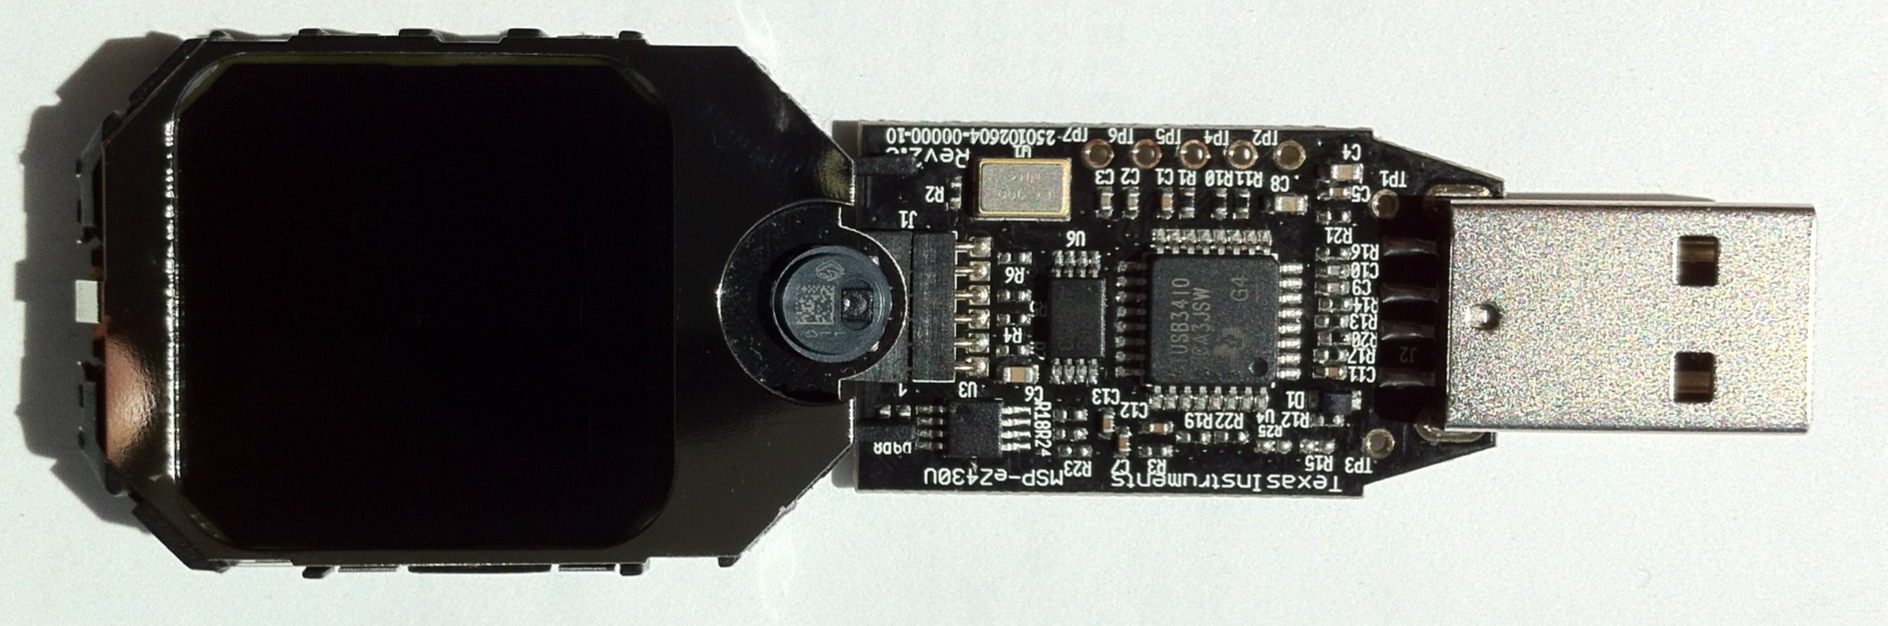
\includegraphics[width=0.8\textwidth]{img/chronos_dongle.jpg}
  \caption{Watch connected to the programming dongle.}
  \label{fig:chronos_dongle}
\end{figure}

Second device is the {\bf USB RF access point dongle}, which can
communicate with the watch over the radio and also forward it's
commands to the PC. One example use is driving PC mouse by moving the
watch, or controlling a presentation with it's buttons. In fact this
dongle is also uses a system-on-chip MCU, which additionally has USB
support. It's architecture is however different and currently
unsupported by TinyOS. Programming it is an interesting future work.

The dongle is shown in figure \ref{fig:chronos_rfdongle}.

\begin{figure}[h]
  \centering
  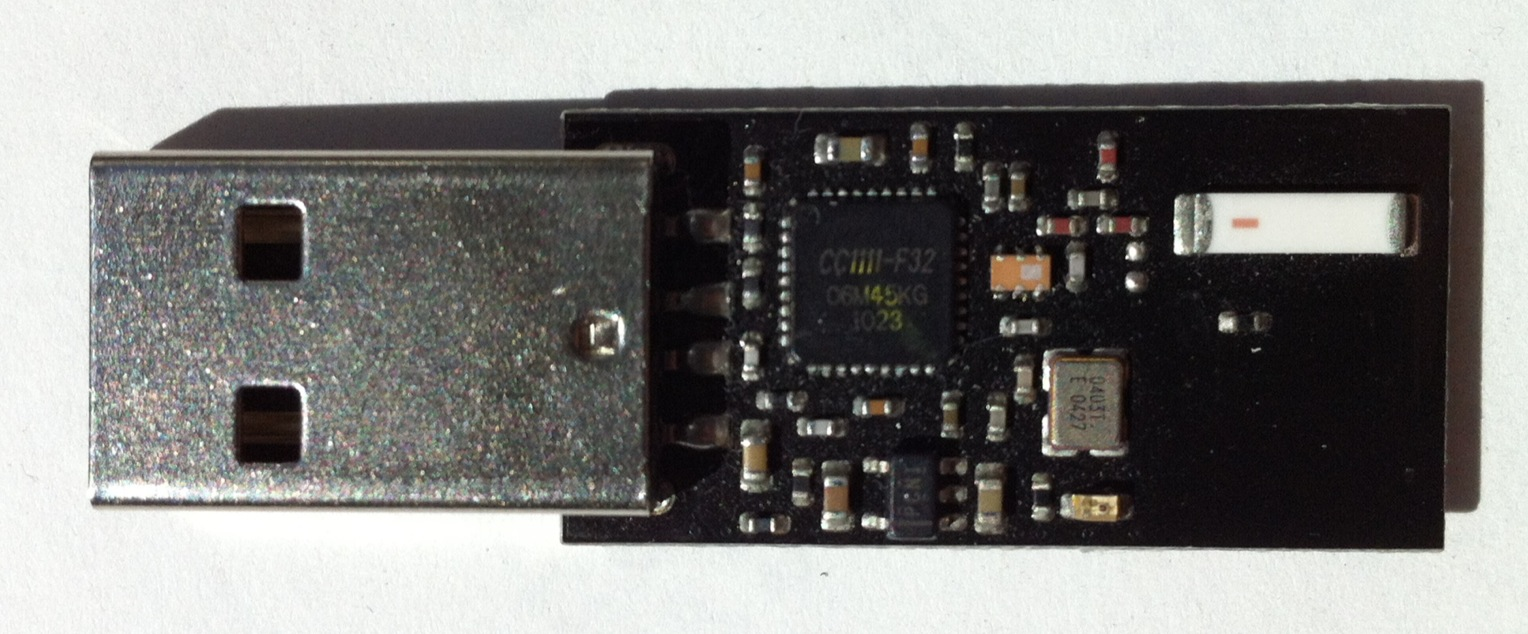
\includegraphics[width=0.6\textwidth]{img/chronos_rfdongle.jpg}
  \caption{USB RF access point dongle.}
  \label{fig:chronos_rfdongle}
\end{figure}

\section{Intended use of the watch}

\subsection{Factory firmware}

TI provides software example that comes preloaded on every watch by
the manufacturer. It provides standard watch functions like time,
date, alarm and stopwatch. Also it shows averaged sensor measurements
altitude, acceleration, battery voltage and temperature. If heart
rate monitor is present it will also display it's readings. For the
radio communication there are few wireless modes:

\begin{itemize}
  \item ACC --- transmit accelerometer motion data.
  \item PPT --- wireless presentation control or bind Chronos
    keys to PC keyboard shortcuts.
  \item Sync --- syncs time and date with PC and calibrates
    temperature and altitude.
\end{itemize}

\subsection{Community use cases}
There are many programs written by technology enthusiasts. Some of the
examples:

\begin{itemize}
  \item wireless door lock --- system of two devices, in addition to beaming two devices it is possible to define a password as a gesture meassured by accelerometer.
  \item flying mouse --- move watch and use it as a PC mouse.
  \item automatic lighting system --- control light bulbs from your watch.
  \item Time-based One Time Password (TOTP) Authenticator --- provides token based authorization system.
\end{itemize}

% Vim settings:
% vim: set textwidth=70:
% vim: set fo+=t:
